\documentclass[]{article}
\usepackage{lmodern}
\usepackage{amssymb,amsmath}
\usepackage{ifxetex,ifluatex}
\usepackage{fixltx2e} % provides \textsubscript
\usepackage[T1]{fontenc}
\usepackage[utf8]{inputenc}
% use upquote if available, for straight quotes in verbatim environments
\IfFileExists{upquote.sty}{\usepackage{upquote}}{}
% use microtype if available
\IfFileExists{microtype.sty}{%
\usepackage[]{microtype}
\UseMicrotypeSet[protrusion]{basicmath} % disable protrusion for tt fonts
}{}
\PassOptionsToPackage{hyphens}{url} % url is loaded by hyperref
\usepackage[unicode=true]{hyperref}
\hypersetup{
            pdfborder={0 0 0},
            breaklinks=true}
\urlstyle{same}  % don't use monospace font for urls
\usepackage{graphicx,grffile}
\makeatletter
\def\maxwidth{\ifdim\Gin@nat@width>\linewidth\linewidth\else\Gin@nat@width\fi}
\def\maxheight{\ifdim\Gin@nat@height>\textheight\textheight\else\Gin@nat@height\fi}
\makeatother
% Scale images if necessary, so that they will not overflow the page
% margins by default, and it is still possible to overwrite the defaults
% using explicit options in \includegraphics[width, height, ...]{}
\setkeys{Gin}{width=\maxwidth,height=\maxheight,keepaspectratio}
\IfFileExists{parskip.sty}{%
\usepackage{parskip}
}{% else
\setlength{\parindent}{0pt}
\setlength{\parskip}{6pt plus 2pt minus 1pt}
}
\setlength{\emergencystretch}{3em}  % prevent overfull lines
\providecommand{\tightlist}{%
  \setlength{\itemsep}{0pt}\setlength{\parskip}{0pt}}
\setcounter{secnumdepth}{0}
% Redefines (sub)paragraphs to behave more like sections
\ifx\paragraph\undefined\else
\let\oldparagraph\paragraph
\renewcommand{\paragraph}[1]{\oldparagraph{#1}\mbox{}}
\fi
\ifx\subparagraph\undefined\else
\let\oldsubparagraph\subparagraph
\renewcommand{\subparagraph}[1]{\oldsubparagraph{#1}\mbox{}}
\fi

% set default figure placement to htbp
\makeatletter
\def\fps@figure{htbp}
\makeatother


\date{}

\begin{document}

Xtext Tutorium

2017, Pierre Bayerl und Tim Schneider

\section[Zusammenfassung]{\texorpdfstring{\protect\hypertarget{anchor}{}{}Zusammenfassung}{Zusammenfassung}}\label{zusammenfassung}

Dieses Dokument spiegelt die ersten Erfahrungen und Schritte wieder, die
uns den Einstieg in Xtext erleichtert haben. Es gibt viele Dokumente,
Einführungen und Kurse zu dem Thema (die meisten sind frei verfügbar).
Ohne sich jedoch die Zeit zu nehmen, die allerersten Schritte zu
verinnerlichen wird man viele Fehlschläge erleiden (insbesondere wo man
was genau eingeben oder einstellen kann oder muss).

\textbf{Abgrenzung}: Dieses Dokument ist keine allumfassende
Dokumentation des Themas. Dazu sind diverse Quellen angegeben (und
entsprechend kommentiert). Darunter ein exzellenter Kurs
\protect\hyperlink{anchor-1}{/1/}, ein aktuelles Buch
\protect\hyperlink{anchor-2}{/2/} und frei verfügbare Dokumente aus dem
Internet (\protect\hyperlink{anchor-3}{/3/},
\protect\hyperlink{anchor-4}{/4/}, \protect\hyperlink{anchor-5}{/5/} und
\protect\hyperlink{anchor-6}{/9/}). Auch werden keine alternativen
Werkzeuge zur Erstellung von DSLs betrachtet (siehe
\protect\hyperlink{anchor-7}{/7/} und
\protect\hyperlink{anchor-8}{/8/}).

\textbf{Ziel}: Es soll demonstriert werden, wie man -- ausgehend von
einem vorhanden Modellierungsgedanken -- die \textbf{Xtext Toolkette
anwenden }kann, um domänenspezifische Modellierungswerkzeuge zu
schaffen. Auch wenn man nicht „programmiert``, soll man eine Idee
bekommen, welche \textbf{Werkzeuganforderungen }durch das Xtext
Framework leicht zu realisieren sind.

\section[Quellen, weiterführende
Literatur]{\texorpdfstring{\protect\hypertarget{anchor-9}{}{}\protect\hypertarget{anchor-10}{}{}Quellen,
weiterführende
Literatur}{Quellen, weiterführende Literatur}}\label{quellen-weiterfuxfchrende-literatur}

\begin{enumerate}
\def\labelenumi{\arabic{enumi}.}
\item
  \protect\hypertarget{anchor-1}{}{}H. Rentz-Reichert (Protos Software):
  "Entwicklung domänenspezifischer Sprachen und Code-Generatoren mit
  Xtext und Xtend" (Kurs, Regensburg, 2017/05).
\item
  \protect\hypertarget{anchor-2}{}{}L. Bettini: "Implementing
  Domain-Specific Languages with Xtext and Xtend - Second Edition``
  (Packt Publishing; 2nd Revised edition, 31. August 2016).
\item
  \protect\hypertarget{anchor-3}{}{}A. Mooij, J. Hooman: "Creating a
  Domain Specific Language (DSL) with Xtext",
  \url{http://www.cs.kun.nl/J.Hooman/DSL/Xtext_DSL_GettingStarted_Neon.pdf}
  (2017/06)
\item
  \protect\hypertarget{anchor-4}{}{}A. Mooij, K. Triantafyllidis, J.
  Hooman: "Advanced Xtext Manual on Modularity",
  \url{http://www.cs.kun.nl/J.Hooman/DSL/AdvancedXtextManual.pdf}
  (2017/06)
\item
  \protect\hypertarget{anchor-5}{}{}Xtext Webseite:
  \url{https://eclipse.org/Xtext/} (2017/06)
\item
  \protect\hypertarget{anchor-11}{}{}Hadi Hariri: „Kotlin for C++
  Developers``, Overload Journal \#139, June 2017;
  \url{https://accu.org/var/uploads/journals/Overload139.pdf}, 2017/06)
\item
  \protect\hypertarget{anchor-7}{}{}\url{https://www.heise.de/developer/artikel/Werkzeuge-fuer-domaenenspezifische-Sprachen-227190.html}
  (2017/06)
\item
  \protect\hypertarget{anchor-8}{}{}\url{https://www.heise.de/developer/artikel/Episode-10-Modellierung-im-Softwarearchitekturumfeld-Teil-1-353335.html}
  und
  \url{https://www.heise.de/developer/artikel/Episode-11-Modellierung-im-Softwarearchitekturumfeld-Teil-2-353355.html}
  (2017/06)
\item
  \protect\hypertarget{anchor-6}{}{}\url{https://www.heise.de/developer/artikel/Eine-eigene-Programmiersprache-mit-Xtext-modellieren-3180566.html}
  (2017/06)
\item
  \protect\hypertarget{anchor-12}{}{}Xtend Sprach-Referenz:
  \url{https://eclipse.org./xtend} (2017/07)
\item
  \protect\hypertarget{anchor-13}{}{}\url{http://www.eclipse.org/Xtext/documentation/310_eclipse_support.html\#templates}
  (2017/07)
\end{enumerate}

\section[Arbeitsumfeld
Eclipse]{\texorpdfstring{\protect\hypertarget{anchor-14}{}{}Arbeitsumfeld
Eclipse}{Arbeitsumfeld Eclipse}}\label{arbeitsumfeld-eclipse}

Um die Übungen in diesem Dokument durchzuführen, muss man Eclipse mit
den notwendigen Xtext Plugins installiert haben (Aktuelle Version:
Oxygen).

Hinweise: \textbf{(1)} Der notwendige Antlr Parser darf nicht mit
Eclipse zusammen verteilt werden (Open Source Lizenz passen nicht
zusammen). Er muss daher ggf. separat installiert werden
(\url{http://download.itemis.de/updates}), sonst will Eclipse ihn bei
jedem neuen Xtext Projekt neu herunterladen. \textbf{(2)} In den
folgenden Abschnitten sind Übungs-Meilensteine mit folgendem Symbol
dargestellt:

\subsection[Eclipse herunterladen, entpacken und
starten]{\texorpdfstring{\protect\hypertarget{anchor-15}{}{}Eclipse
herunterladen, entpacken und
starten}{Eclipse herunterladen, entpacken und starten}}\label{eclipse-herunterladen-entpacken-und-starten}

Lade das Paket „Eclipse Modeling`` auf der Seite
\url{http://www.eclipse.org/downloads/packages/} herunter. Nachdem
herunterladen empfiehlt es sich das Archiv zu entpacken und in das
gewünschte Verzeichnis zu entpacken.

root@xtext:\textasciitilde{}/Download\# ls

eclipse-modeling-oxygen-3a-linux-gtk-x86\_64.tar.gz

root@xtext:\textasciitilde{}/Download\# tar xzf
eclipse-modeling-oxygen-3a-linux-gtk-x86\_64.tar.gz

root@xtext:\textasciitilde{}/Download\# mv eclipse /opt/

root@xtext:\textasciitilde{}/Download\# /opt/eclipse/eclipse \&

\subsection[Eclipse starten und Xtext
installieren]{\texorpdfstring{\protect\hypertarget{anchor-16}{}{}Eclipse
starten und Xtext
installieren}{Eclipse starten und Xtext installieren}}\label{eclipse-starten-und-xtext-installieren}

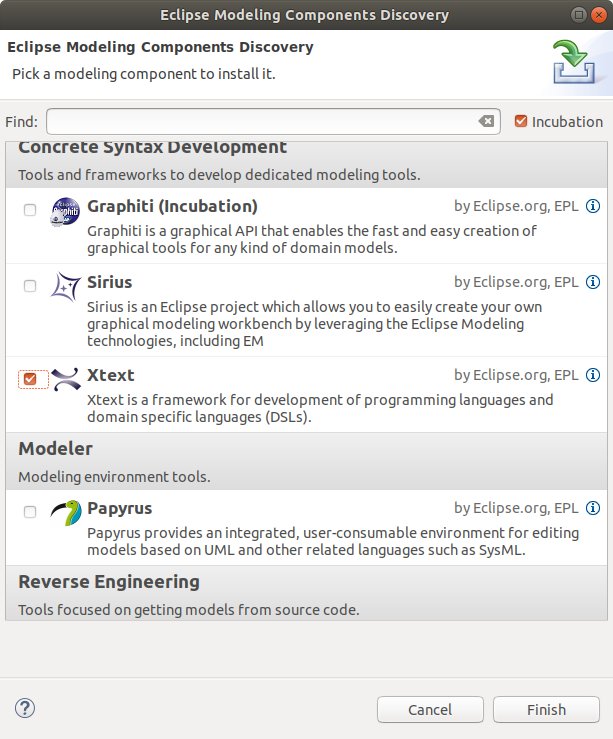
\includegraphics[width=3.73660in,height=4.50470in]{./Pictures/1000020100000265000002E3C3D1AD84052DE450.png}Um
Xtext zu installieren muss im „Help`` Menü „Install Modeling
Components`` ausgewählt werden. Im folgendem Dialog wählt man dann Xtext
aus und bestätigt mit „Finish``. Ist die Installation erfolgreich, wird
ein neustart der Entwicklungsumgebung verlangt.

\section[Eine erste
Grammatik]{\texorpdfstring{\protect\hypertarget{anchor-17}{}{}Eine erste
Grammatik}{Eine erste Grammatik}}\label{eine-erste-grammatik}

\begin{figure}
\centering
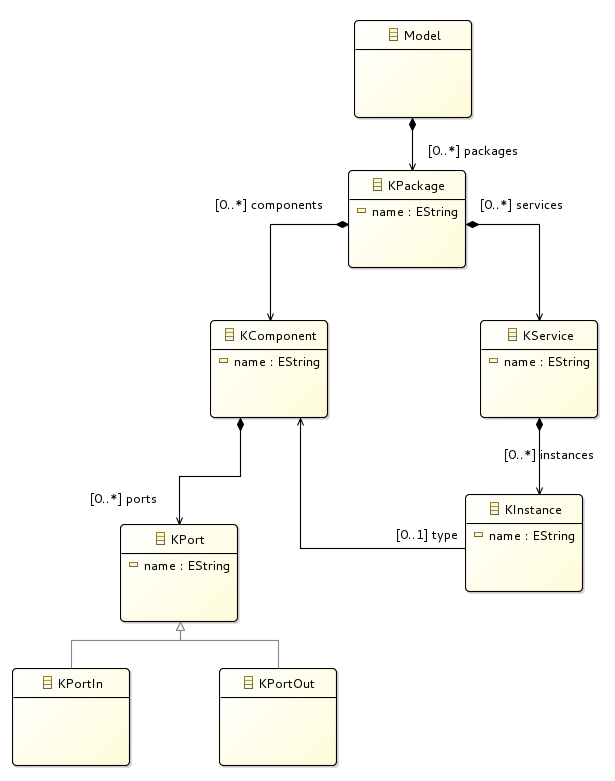
\includegraphics[width=5.12520in,height=6.50830in]{./Pictures/10000201000002670000030DD0AB9EF4251EDB4D.png}
\caption{Illustration 1: Ziel-Metamodell}
\end{figure}

\emph{\textbf{Ziel dieser Übung }}ist es, eine Grammatik für obigen
Sachverhalt zu definieren: Ein \textbf{Modell}, dass \textbf{Packages
}beinhaltet. Jedes Package wiederum kann \textbf{Komponenten definieren
und instanziieren}. Weiter kann eine Komponentendefinition
\textbf{Eingabe und Ausgabe Ports }beinhalten.

Man soll sich dabei an die Syntax der Grammatik gewöhnen. Diese ist das
Mittel, um das Metamodell für die Struktur des zu definierenden Modells
zu spezifizieren.

\subsection{}\label{section}

\subsection[Neues Xtext Projekt
anlegen]{\texorpdfstring{\protect\hypertarget{anchor-18}{}{}Neues Xtext
Projekt
anlegen}{Neues Xtext Projekt anlegen}}\label{neues-xtext-projekt-anlegen}


\includegraphics[width=0.98350in,height=0.98350in]{./Pictures/1000020100000080000000807EA91CDFA7B7F397.png}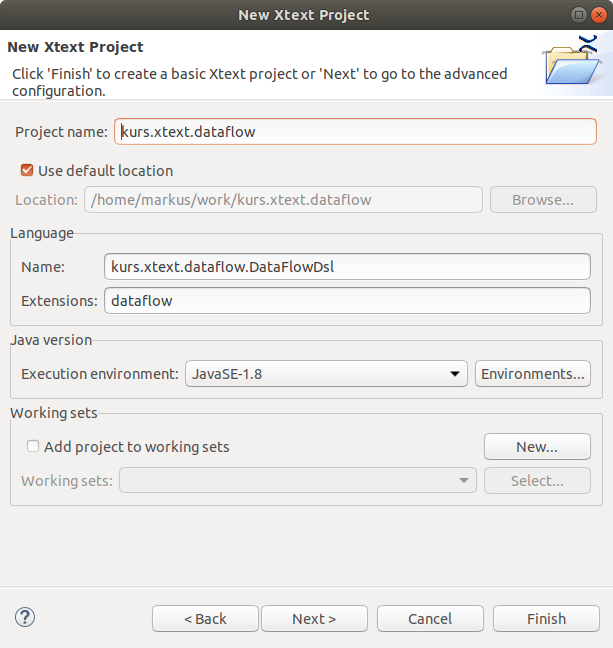
\includegraphics[width=4.24090in,height=5.15550in]{./Pictures/10000201000002650000028845D817BB3C722F32.png}

\begin{enumerate}
\def\labelenumi{\arabic{enumi}.}
\tightlist
\item
  Im Menü „File`` - „New`` - „Project`` auswählen
\item
  Im folgendem Dialog „Xtext Project`` auswählen und mit „Next``
  bestätigten
\item
  Nun 
\end{enumerate}

\begin{itemize}
\item
  \begin{itemize}
  \item
    „\textbf{Project name}``=``kurs.xtext.dataflow``
  \item
    „\textbf{Name}=`` kurs.xtext.dataflow.DataFlowDsl``
  \item
    „\textbf{Extensions}``=``dataflow`` eingeben

    und „\textbf{Next}`` klicken.
  \end{itemize}
\end{itemize}

\begin{enumerate}
\def\labelenumi{\arabic{enumi}.}
\tightlist
\item
  Im nächsten Dialog besteht nun die Möglichkeit zwischen den „Facets``
  auszuwählen. Bei dem Punkt „Prefered Build System`` Maven auswählen,
  da dies für späteres bauen der DSL benötigt wird. Folgende
  Einstellungen werden empfohlen, um die Besipiele in diesem Tutorium
  anzuwenden. Die Warnung „Maven integration for eclipse (m2e)`` sollte
  nicht ignoriert werden und einfach über das Menü „Help`` - „Install
  New Software`` - „All Availabe Sites`` - „m2e`` nachinstalliert
  werden. Auch hier wieder mit einem Neustart bestätigen.
\end{enumerate}

Es entstehen mehrerer Projekte (Details: siehe
\protect\hyperlink{anchor-3}{/3/}), von denen für uns zunächst nur das
erste von Interesse ist. Es wird eine Beispiel-Grammatikdefinition
erstellt (Hello World) und im Editor geöffnet.

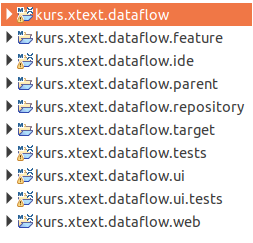
\includegraphics[width=2.63540in,height=2.53110in]{./Pictures/10000201000000FD000000F33F19609DDE80FED7.png}

\subsection[Xtext Projekt übersetzen und Sprache
ausprobieren]{\texorpdfstring{\protect\hypertarget{anchor-19}{}{}Xtext
Projekt übersetzen und Sprache
ausprobieren}{Xtext Projekt übersetzen und Sprache ausprobieren}}\label{xtext-projekt-uxfcbersetzen-und-sprache-ausprobieren}

\begin{enumerate}
\def\labelenumi{\arabic{enumi}.}
\tightlist
\item
  In die Grammatik mittels „Rechts-Klick``: \textbf{Run As / Generate
  Xtext Artifacts} 
\item
  Im Menu: \textbf{Run / Debug Configurations \ldots{}}
\end{enumerate}

\begin{itemize}
\item
  \begin{itemize}
  \item
    
\includegraphics[width=0.39290in,height=0.37360in]{./Pictures/10000201000000150000001454902A3E6367315A.png}„\textbf{Eclipse
    Application}`` anwählen
  \item
    Icon „\textbf{New Launch Configuration}`` klicken 
  \item
    Optional:

    \begin{itemize}
    \tightlist
    \item
      „Name`` anpassen und
    \item
      die „Location`` anpassen (Arbeits Workspace zum Probieren der
      neuen Plugins)
    \end{itemize}
  \item
    „\textbf{Debug}`` klicken
  \end{itemize}
\end{itemize}

Nun geht eine neue Eclipse-Instanz auf. Hier kann man nun die neue
Sprache ausprobieren:

\begin{enumerate}
\def\labelenumi{\arabic{enumi}.}
\item
  Im „Package Explorer``: \textbf{New Project} klicken.
\item
  „\textbf{Java Project}`` wählen und entsprechend ein Projekt anlegen
  (z.B. „Test1``) - Es ist dabei jedoch irrelevant, ob man hier Java
  oder z.B. C++ wählt.
\item
  In diesem Projekt nun einen \textbf{Ordner „model`` anlegen:\\
   }
\item
  In diesem Ordner nun eine Modelldatei anlegen: \textbf{New / File} mit
  „\textbf{File Name}``=``test1.\emph{dataflow}`` und „\textbf{Finish}``
  klicken.
\item
  Die folgende Frage mit „\textbf{Yes}`` beantworten:

  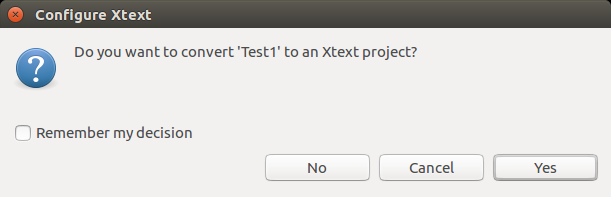
\includegraphics[width=4.36890in,height=1.40830in]{./Pictures/1000020100000263000000C5AC8B604E35219E41.png}
\end{enumerate}


\includegraphics[width=0.98350in,height=0.98350in]{./Pictures/1000020100000080000000807EA91CDFA7B7F397.png}Nun
können Sie die Hallo Welt Grammatik ausprobieren\\
(probieren Sie CTRL-Space aus) und geben Sie dann folgendes Beispiel
ein:

\textbf{Hello} Pierre!

\textbf{Hello} Tim!

\textbf{Hello} Markus!

\subsection[Eine eigene Grammatik eingeben (Teil
1)]{\texorpdfstring{\protect\hypertarget{anchor-20}{}{}Eine eigene
Grammatik eingeben (Teil
1)}{Eine eigene Grammatik eingeben (Teil 1)}}\label{eine-eigene-grammatik-eingeben-teil-1}

Eine Grammatik beschreibt die Syntax (quasi ohne Semantik) und erzeugt
intern ein ecore-Modell, dass man sich anschauen kann. Der „Master`` ist
jedoch die Grammatik (für die Wartung).

Hinweis: Es ist auch möglich, eine Grammatik aus einem ecore-Modell zu
generieren (via Eclipse Wizard).

\subsubsection[Basis Knoten für das
Modell]{\texorpdfstring{\protect\hypertarget{anchor-21}{}{}Basis Knoten
für das
Modell}{Basis Knoten für das Modell}}\label{basis-knoten-fuxfcr-das-modell}

\begin{itemize}
\tightlist
\item
  Die erste Regel in der Grammatik („Modell`` in der Hallo Welt
  Grammatik) beschreibt den Startpunkt des Modells (das Wurzelelement).
\item
  Statt der Modellelemente vom Typ „Greeting`` wollen wir nun
  „KPackage``-Elemente definieren (vgl. ).
\item
  Siehe auch: \protect\hyperlink{anchor-3}{/3/}
\end{itemize}

\subsubsection[Attribute,
Komposition]{\texorpdfstring{\protect\hypertarget{anchor-22}{}{}Attribute,
Komposition}{Attribute, Komposition}}\label{attribute-komposition}

Ein KPackage wiederum soll eine Komposition aus KComponent und KService
Elementen darstellen:

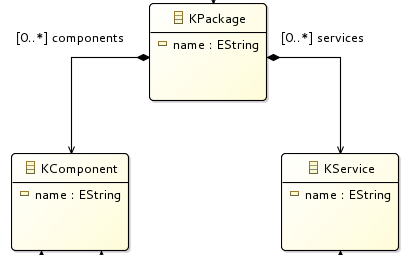
\includegraphics[width=3.45830in,height=2.12520in]{./Pictures/100002010000019F000000FFAC91D652B890571C.png}

KPackage: 'package' name=ID '\{'

(

components += KComponent \textbar{}

services += KService

)*

'\}'

;

\begin{itemize}
\item
  'package', '\{', '\}'

  \begin{itemize}
  \tightlist
  \item
    ist jeweils ein \textbf{Schlüsselwort}
  \end{itemize}
\item
  name=ID

  \begin{itemize}
  \tightlist
  \item
    „name`` ist \textbf{Attribut }im Metamodell (Das Attribut „name``
    hat eine Sonderbedeutung: Es beschreibt den Namen des Elements).
  \item
    „=`` bedeutet: es ist ein \emph{\textbf{Wert}}\textbf{ }(keine Liste
    von Werten)
  \item
    \textbf{ID ist ein Terminal} (siehe \textbf{grammar}
    kurs.xtext.dataflow.DataFlowDsl \textbf{with}
    org.eclipse.xtext.common.Terminals - „F3`` auf Terminals klicken, um
    die Terminals zu sehen)
  \end{itemize}
\item
  components += KComponent

  \begin{itemize}
  \tightlist
  \item
    „components`` ist ein \textbf{Attribut }im Metamodell
  \item
    „+=`` bedeutet es ist eine \emph{\textbf{Liste}}, an die hinzugefügt
    wird
  \item
    „KComponent`` und „KService`` sind Definitionen analog zu einem
    „KPackage`` 
  \end{itemize}
\item
  ( ... \textbar{} ... )*

  \begin{itemize}
  \tightlist
  \item
    Alles innerhalb der Klammer ist 0 bis n Mal erlaubt („+`` statt „*``
    bedeutet 1 bis n Mal).
  \item
    „\textbar{}`` ist hier ein „oder``
  \end{itemize}
\end{itemize}

Folgende Eingaben sollen möglich werden:

\textbf{package} test1 \{


\includegraphics[width=0.98350in,height=0.98350in]{./Pictures/1000020100000080000000807EA91CDFA7B7F397.png}\textbf{Component}
PC \{

\}

\textbf{Component} DF \{

\}

\textbf{service} MyService \{

\}

\}

→ Testen Sie Ihre Grammatik (wie oben beschrieben: „\textbf{Run As /
Xtext Artifacts}`` und dann die angelegte Debugkonfiguration via „Icon``
in der Iconleiste starten).

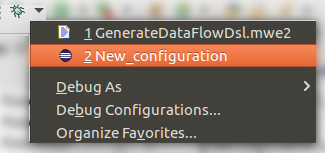
\includegraphics[width=3.38540in,height=1.59370in]{./Pictures/100002010000014500000099ABA38A95A85F29E5.png}

\subsection[Eine eigene Grammatik eingeben (Teil
2)]{\texorpdfstring{\protect\hypertarget{anchor-23}{}{}Eine eigene
Grammatik eingeben (Teil
2)}{Eine eigene Grammatik eingeben (Teil 2)}}\label{eine-eigene-grammatik-eingeben-teil-2}

Es folgen nun weitere Möglichkeiten, um das Metamodell zu spezifizieren.

Weitere Informationen entnehmen Sie den Referenzen. Weiter ist eine
Offline Hilfe in Eclipse integriert: „Help / Help Contents``

\subsubsection[Referenzen]{\texorpdfstring{\protect\hypertarget{anchor-24}{}{}Referenzen}{Referenzen}}\label{referenzen}

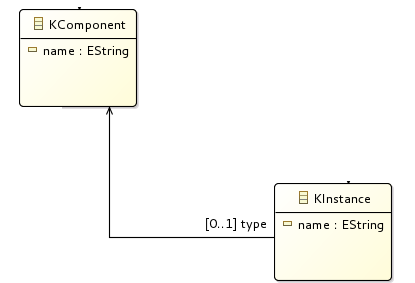
\includegraphics[width=3.45830in,height=2.35830in]{./Pictures/100002010000019F0000011B523F6AF86839FE43.png}

KInstance: 'instance' name=ID ':' type={[}\emph{KComponent}{]};

\begin{itemize}
\item
  type={[}KComponent{]}

  \begin{itemize}
  \tightlist
  \item
    „type`` ist ein Attribut (ein Referenzattribut) im Metamodell
  \item
    „{[}KComponent{]}`` ist eine \textbf{Referenz} auf ein „KComponent``
  \item
    Siehe auch: \protect\hyperlink{anchor-1}{/1/},
    \protect\hyperlink{anchor-3}{/3/}, \protect\hyperlink{anchor-2}{/2/}
  \end{itemize}
\end{itemize}

\subsubsection{}\label{section-1}

\subsubsection[Vererbung]{\texorpdfstring{\protect\hypertarget{anchor-25}{}{}Vererbung}{Vererbung}}\label{vererbung}

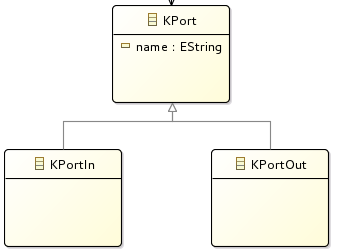
\includegraphics[width=2.82520in,height=2.09170in]{./Pictures/1000020100000153000000FB3A29A3A8CA4988F4.png}

KPort:

KPortIn\textbar{}KPortOut

;

KPortIn:

'port\_in' name=ID '\{'

'\}'

;

KPortOut:

'port\_out' name=ID '\{'

'\}'

;

\begin{itemize}
\item
  „Base: SpecialA\textbar{}SpecialB;``

  \begin{itemize}
  \tightlist
  \item
    Definiert eine Basisklasse ausgehend von den Spezialisierungen.
  \item
    Gemeinsame Attribute wandern dabei automatisch in die Basisklasse
    (hier: „name``)
  \item
    Siehe auch: \protect\hyperlink{anchor-1}{/1/},
    \protect\hyperlink{anchor-3}{/3/}, \protect\hyperlink{anchor-2}{/2/}
  \end{itemize}
\end{itemize}

\subsubsection[Editor]{\texorpdfstring{\protect\hypertarget{anchor-26}{}{}Editor}{Editor}}\label{editor}

Nun müssen Sie noch den Komponenten (KComponent) Ports und den Services
(KService) Instanzen hinzugefügen (vgl. ).

Probieren Sie nun Ihre Grammatik aus (Abschnitte
\protect\hyperlink{anchor-24}{4.4.1},
\protect\hyperlink{anchor-25}{4.4.2},
\protect\hyperlink{anchor-26}{4.4.3}):


\includegraphics[width=0.98350in,height=0.98350in]{./Pictures/1000020100000080000000807EA91CDFA7B7F397.png}\textbf{package}
test1 \{

\textbf{Component} PC \{

\textbf{port\_in} in \{\}

\textbf{port\_out} out \{\}

\}

\textbf{Component} DF \{

\textbf{port\_in} in \{\}

\textbf{port\_out} out \{\}

\textbf{port\_out} debug \{\}

\}

\textbf{service} MyService \{

\textbf{instance} pc : PC

\textbf{instance} df : DF

\}

\}

Die Eingaben sind analog ebenso als Baum verfügbar und zeitgleich
editierbar (Die Datei mit „\textbf{Open With...}`` „\textbf{Sample Ecore
Model Editor}`` öffnen, verändern, speichern):

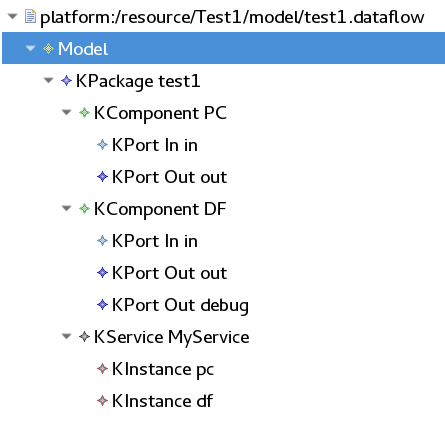
\includegraphics[width=3.39090in,height=3.21610in]{./Pictures/10000201000001BD000001A641C76BF87A14C60B.png}

\subsubsection{Mehr Grammatik\ldots{}}\label{mehr-grammatik}

Die Grammatik bietet noch ein paar mehr Facetten, die in diesem Rahmen
nicht angesprochen werden. Siehe dazu die Xtext Hilfe in Eclipse, oder
\protect\hyperlink{anchor-2}{/2/}, \protect\hyperlink{anchor-3}{/3/},
\protect\hyperlink{anchor-5}{/5/}.

Hervorzuheben sind

\begin{itemize}
\tightlist
\item
  \textbf{Optionale Teile }der Grammatik mittels „?``
\item
  \textbf{Enums }(deren erster Zustand eingenommen wird, wenn die
  Variable optional ist, und nicht gesetzt wurde).
\end{itemize}

\subsubsection[Option: Auto
Formatting]{\texorpdfstring{\protect\hypertarget{anchor-27}{}{}Option:
Auto Formatting}{Option: Auto Formatting}}\label{option-auto-formatting}

Hinweis: Wenn Sie in der Baumansicht neue Objekte anlegen und
abspeichern, werden Sie sehen, dass der damit erzeugte Text keine
Zeilenumbrüche besitzt. Auch das Auto-Formatting von Eclipse erzeugt
dieses Problem (\textbf{CTRL-SHIFT-F} im Text Editor; mit CTRL-Z
rückgängig machen). Dieses Verhalten kann man einfach umkonfigurieren,
indem man sich um „Xtext Formatting`` kümmert:

\begin{itemize}
\item
  Legen Sie eine neue Java Klasse
  „\textbf{kurs.xtext.dataflow.formatting}.\textbf{MyFormatter}`` im
  Ihrem Projekt mit der Grammatik an, das von
  „\textbf{org.eclipse.xtext.formatting.impl.AbstractDeclarativeFormatter}``
  abgeleitet ist.

  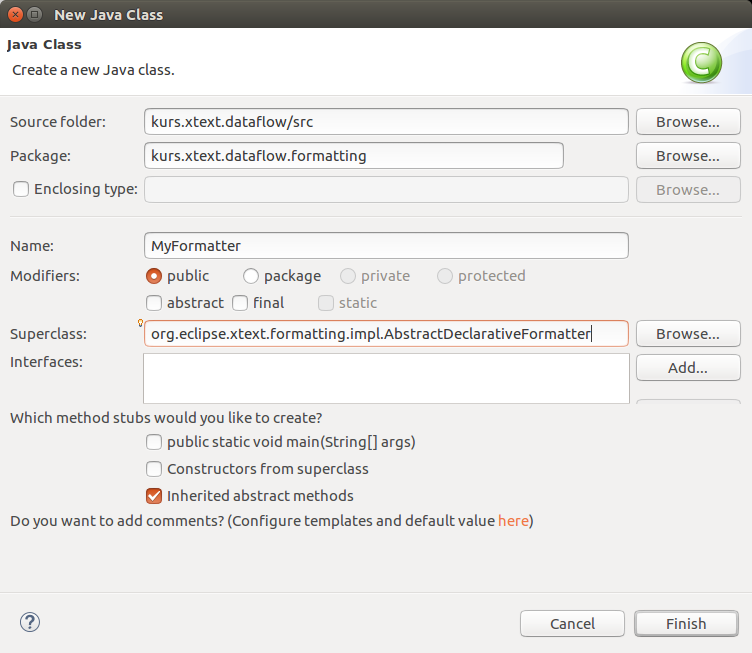
\includegraphics[width=5.89650in,height=5.12010in]{./Pictures/10000201000002F00000028DA25B000046F4964A.png}
\item
  Geben Sie hier folgenden Code ein, um u.a. das Verhalten um „\{`` und
  „\}`` zu steuern:
\end{itemize}

\textbf{package} kurs.xtext.dataflow.formatting;

\textbf{import} org.eclipse.xtext.Keyword;

\textbf{import}
org.eclipse.xtext.formatting.impl.AbstractDeclarativeFormatter;

\textbf{import} org.eclipse.xtext.formatting.impl.FormattingConfig;

\textbf{import} org.eclipse.xtext.util.Pair;

\textbf{import} kurs.xtext.dataflow.services.DataFlowDslGrammarAccess;

\textbf{public} \textbf{class} MyFormatter \textbf{extends}
AbstractDeclarativeFormatter \{

@Override

\textbf{protected} \textbf{void} configureFormatting(FormattingConfig
config) \{

DataFlowDslGrammarAccess ga = (DataFlowDslGrammarAccess)
getGrammarAccess();

\textbf{for} (Pair\textless{}Keyword, Keyword\textgreater{} pair :
ga.findKeywordPairs("\{", "\}")) \{

config.setLinewrap().after(pair.getFirst());

config.setIndentationIncrement().after(pair.getFirst());

config.setLinewrap().before(pair.getSecond());

config.setIndentationDecrement().before(pair.getSecond());

config.setLinewrap().after(pair.getSecond());

\}

config.setLinewrap(1, 1, 1).after(ga.getKInstanceRule());

\}

\}

\begin{itemize}
\tightlist
\item
  Diesen neuen Formatter müssen Sie nun noch anmelden. Geben Sie in der
  Datei kurs.xtext.dataflow.DataFlowDslRuntimeModule.xtend folgenden
  Code ein:
\end{itemize}

\textbf{override} bindIFormatter() \{

MyFormatter

\}

(Hinweis: Xtend ist eine Xtext Sprache, die direkt in Java Code
umgewandelt wird. Jede Xtend Klasse kann auch in Java geschrieben
werden. Xtend bietet viele Eigenschaften, die insbesondere
Codegenerierung und kompakte Schreibweisen erleichtern -- die man auch
in anderen modernen Hype-Sprachen -- wie z.B. Kotlin o.ä. wiederfindet;
vgl. z.B. \protect\hyperlink{anchor-11}{/6/}.

\begin{itemize}
\tightlist
\item
  Starten Sie Ihre Arbeits Workbench nun neu und probieren Sie den neuen
  Formatter aus (CTRL-SHIFT-F).
\end{itemize}

Weitere Informationen: \protect\hyperlink{anchor-1}{/1/} und JavaDoc von
FormattingConfig
(\url{http://download.eclipse.org/modeling/tmf/xtext/javadoc/2.3/org/eclipse/xtext/formatting/impl/FormattingConfig.html},
2017/06).

\subsubsection{Option: Meta Modell
visualisieren}\label{option-meta-modell-visualisieren}

Man kann das Ecore Metamodell, das durch die Grammatik definiert wird,
visualisieren: siehe \protect\hyperlink{anchor-3}{/3/}, Kapitel „3.1.3
Optional: Ecore diagram``. Weiter kann man die Grammatik selbst
graphisch darstellen: siehe \protect\hyperlink{anchor-3}{/3/}, Kapitel
„3.1.2 Construct grammar of DSL``, Abschnitt „Optional: View Diagram of
Xtext Grammar``.

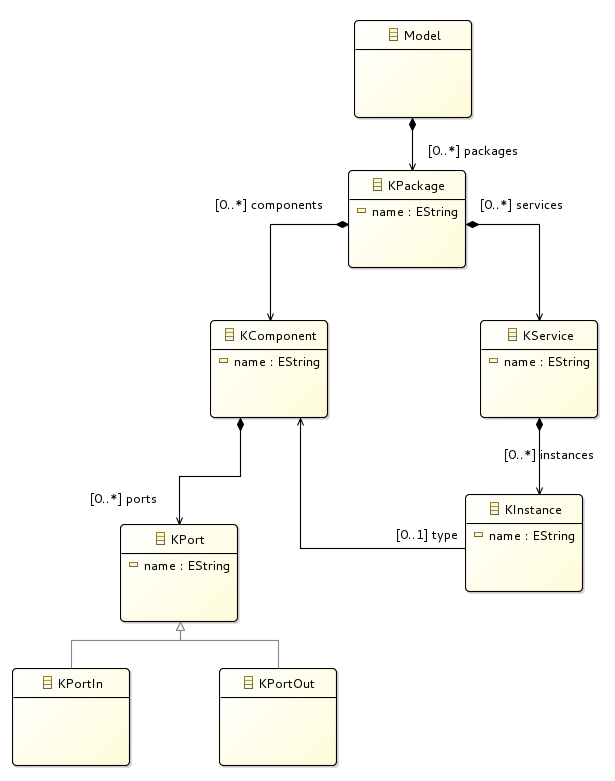
\includegraphics[width=3.48070in,height=4.41890in]{./Pictures/10000201000002670000030DFC51453B7F2AE519.png}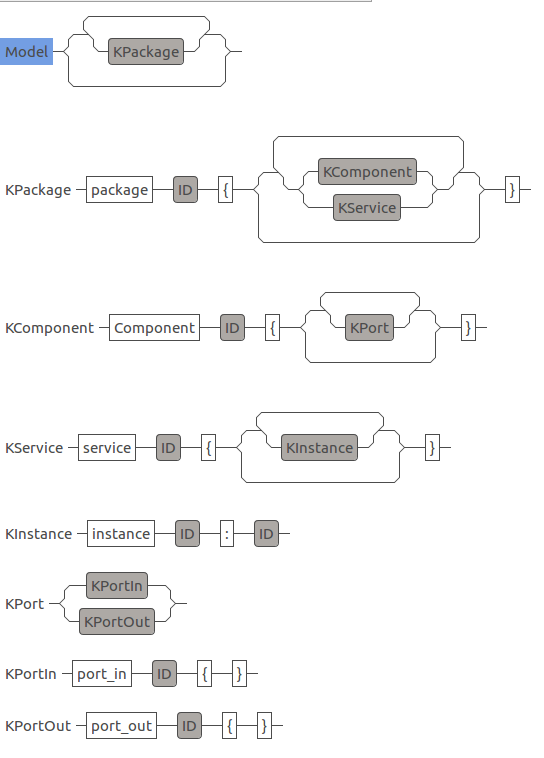
\includegraphics[width=3.16730in,height=4.41340in]{./Pictures/1000020100000220000002F6794AA4A4B50FC707.png}

Links: Erzeugtes Ecore Diagramm („Initialize Ecore Diagram ...``)

Rechts: Syntax Graph der Grammatik (Window/Show
View/Other\ldots{}/Xtext/Xtext Syntax Graph)

\section[Validierung]{\texorpdfstring{\protect\hypertarget{anchor-28}{}{}\protect\hypertarget{anchor-29}{}{}Validierung}{Validierung}}\label{validierung}

Sie können nun Ihre Grammatik validieren. Hier kann durch explizite
programmatische Regeln das eingegeben Modell geprüft werden. Fehler oder
Warnungen werden an Modellelementen angehängt und werden im Eclipse
Editor angezeigt. Weitere Informationen (u.a.): siehe
\protect\hyperlink{anchor-3}{/3/}.

In \protect\hyperlink{anchor-1}{/1/} wurde suggeriert, in die Grammatik
möglichst wenig Semantik einzubauen (um diese einfach zu halten). Also
z.B. lieber „*`` statt „+`` und entsprechende Semantik in die
Validierung zu stecken.

\subsection[Validierung:
Beispiel]{\texorpdfstring{\protect\hypertarget{anchor-30}{}{}\protect\hypertarget{anchor-31}{}{}Validierung:
Beispiel}{Validierung: Beispiel}}\label{validierung-beispiel}

Öffnen Sie die Datei
kurs.xtext.dataflow.validation.DataFlowDslValidator.xtend, kommentieren
Sie den auskommentierten Teil ein und modifizieren Sie ihn:


\includegraphics[width=0.98350in,height=0.98350in]{./Pictures/1000020100000080000000807EA91CDFA7B7F397.png}\textbf{package}
kurs.xtext.dataflow.validation

\textbf{import} org.eclipse.xtext.validation.Check

\textbf{import} kurs.xtext.dataflow.dataFlowDsl.KComponent

\textbf{import} kurs.xtext.dataflow.dataFlowDsl.DataFlowDslPackage

\textbf{class} DataFlowDslValidator \textbf{extends}
AbstractDataFlowDslValidator \{

\textbf{public} \textbf{static} \textbf{val} \emph{INVALID\_NAME} =
'invalidName'

@Check

\textbf{def} checkComponentStartsWithCapital(KComponent c) \{

\textbf{if} (!Character.\emph{isUpperCase}(c.name.charAt(0))) \{

warning('Name should start with a capital',

DataFlowDslPackage.Literals.\emph{KCOMPONENT\_\_NAME},

\emph{INVALID\_NAME})

\}

\}

\}

Probieren Sie die Regel im Editor aus.

Hinweis:

\begin{itemize}
\tightlist
\item
  Eine Regel wird hier durch die Annotation „@Check`` als Regel markiert
  und bekommt ein Modellelement als Eingabe.
\item
  Die Regel wird bei der Eingabe geprüft (@Check bietet hier noch
  weitere Optionen für langsame Checks: während der Eingabe, beim
  Speichern und auf Anfrage -- siehe
  org.eclipse.xtext.validation.CheckType; „F3`` auf @Check anwenden)
\item
  Die Regel betrifft Modellelemente vom Typ „KComponent``
  (Parameterübergabe). An diesen Elementen wird der Fehler auch
  aufgehängt.
\item
  Die hier verwendete Sprache ist Xtend. Alternativ kann die Regel auch
  in Java programmiert werden.
\item
  Eine Regel kann „errors``, „warnings`` und „infos`` erzeugen, welche
  über IDs identifizierbar werden (bei uns „INVALID\_NAME``) - damit
  kann man später Hotfixes mit den Meldungen verknüpfen. Weiter können
  Stringinformationen an die Hotfixes mit übergeben werden.
\end{itemize}

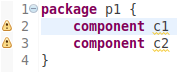
\includegraphics[width=1.84370in,height=0.75000in]{./Pictures/10000201000000B1000000483B963938C77E8851.png}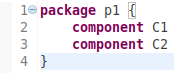
\includegraphics[width=1.81260in,height=0.76020in]{./Pictures/10000201000000AE00000049360C389AF76C863A.png}

\subsection[Option:
Quickfixes]{\texorpdfstring{\protect\hypertarget{anchor-32}{}{}Option:
Quickfixes}{Option: Quickfixes}}\label{option-quickfixes}

Öffnen Sie
kurs.xtext.dataflow.ui.quickfix.DataFlowDslQuickfixProvider.xtend im
\textbf{ui-Projekt}. Hier können Sie Quickfixes implementieren.

Beispiel (der in der Datei schon vorhandene Beispiel-Code kann in
unserem Beispiel quasi ohne Anpassung aktiviert werden):

@Fix(DataFlowDslValidator.\emph{INVALID\_NAME})

\textbf{def} capitalizeName(Issue issue, IssueResolutionAcceptor
acceptor) \{

acceptor.accept(issue, 'Capitalize name', 'Capitalize the name.',
'upcase.png') {[}

context \textbar{}

\textbf{val} xtextDocument = context.xtextDocument

\textbf{val} firstLetter = xtextDocument.get(issue.offset, 1)

xtextDocument.replace(issue.offset, 1, firstLetter.toUpperCase)

{]}

\}

Im vorgegeben Beispiel bekommt der Quickfix direkten Zugriff auf den
Text, auf den er angewendet werden soll. Über die ID „INVALID\_NAME``
ist der Quickfix mit einem Validierungsproblem verknüpft.

Alternativ kann man auch den Zugriff auf das Modellelement bekommen, das
das Validierungsproblem verursacht hat:

@Fix(DataFlowDslValidator.\emph{INVALID\_NAME})

\textbf{def} capitalizeName2(Issue issue, IssueResolutionAcceptor
acceptor) \{

acceptor.accept(issue, 'Capitalize name 2', 'Capitalize the name.',
'upcase.png') {[}

element, context \textbar{}

\textbf{val} c=element \textbf{as} KComponent

c.name = c.name.\emph{toFirstUpper}

{]}

\}

Hinweis:

\begin{itemize}
\tightlist
\item
  Die Annotation „Fix`` markiert die Methode als Quickfix und verknüpft
  diesen Quickfix mit einem Validierungsproblem über eine entsprechende
  eindeutige ID.
\item
  Weitere Anmerkungen zu Xtend (z.B. Bedeutung von „val``, „as``,
  \ldots{}) siehe Kapitel \protect\hyperlink{anchor-33}{6}.
\end{itemize}

\section[Code
Generierung]{\texorpdfstring{\protect\hypertarget{anchor-33}{}{}\protect\hypertarget{anchor-34}{}{}Code
Generierung}{Code Generierung}}\label{code-generierung}

Die Codegenerierung wird bei Xtext typischerweise in Xtend programmiert.

Arbeitet man in der Arbeitsworkbench im Debug Modus, kann man die Code
Generierung normalerweise ohne Neustart dieser Workbench anpassen.

Die Code Generierung in der Arbeitsworkbench für eine Modelldatei
entspricht dem Compilieren einer Java Datei in einem Java Projekt.
Normalerweise passiert das Code Generieren beim Abspeichern der
Modelldatei (auto-compile).

\subsection[Code Generierung:
Beispiel]{\texorpdfstring{\protect\hypertarget{anchor-35}{}{}Code
Generierung:
Beispiel}{Code Generierung: Beispiel}}\label{code-generierung-beispiel}

Öffnen Sie kurs.xtext.dataflow.generator.DataFlowDslGenerator.xtend.
Hier kann ein erster Code Generator implementiert werden:

Hier bekommt man insbesondere die Modellinformation über eine sogenannte
Ressource (Parameter \textbf{resource}) und eine Möglichkeit mit dem
Dateisystem (Parameter \textbf{fsa})zu interagieren.

\textbf{override} \textbf{void} doGenerate(Resource \textbf{resource},
IFileSystemAccess2 \textbf{fsa},

IGeneratorContext context) \{

//
-\/-\/-\/-\/-\/-\/-\/-\/-\/-\/-\/-\/-\/-\/-\/-\/-\/-\/-\/-\/-\/-\/-\/-\/-\/-\/-\/-\/-\/-\/-\/-\/-\/-\/-\/-\/-\/-\/-\/-\/-\/-\/-

// Option 1:

\textbf{var} txt = ""

\textbf{for} (obj: resource.allContents.\emph{toIterable}) \{

\textbf{if} (obj \textbf{instanceof} KComponent) \{ // inside this "if"
\emph{obj} is a KComponent

\textbf{if} (txt.length\textgreater{}0) txt = txt + ", "

txt = txt + obj.name;

\}

\}

fsa.generateFile('Components1.\emph{txt}', 'Component declarations: ' +
txt);

//
-\/-\/-\/-\/-\/-\/-\/-\/-\/-\/-\/-\/-\/-\/-\/-\/-\/-\/-\/-\/-\/-\/-\/-\/-\/-\/-\/-\/-\/-\/-\/-\/-\/-\/-\/-\/-\/-\/-\/-\/-\/-\/-

// Option 2:

fsa.generateFile('Components2.\emph{txt}', 'Component declarations: ' +

resource.allContents

.\emph{filter}{[} obj \textbar{} obj \textbf{instanceof} KComponent{]}

.\emph{map}{[} obj \textbar{} \textbf{return} (obj \textbf{as}
KComponent).name {]}

.\emph{join}(', '))

//
-\/-\/-\/-\/-\/-\/-\/-\/-\/-\/-\/-\/-\/-\/-\/-\/-\/-\/-\/-\/-\/-\/-\/-\/-\/-\/-\/-\/-\/-\/-\/-\/-\/-\/-\/-\/-\/-\/-\/-\/-\/-\/-

// Option 3:

fsa.generateFile('Components3.\emph{txt}', 'Component declarations: ' +

resource.allContents.\emph{filter}(KComponent).\emph{map}{[}name{]}.\emph{join}(',
'))

\}

Es wird auf drei verschiedene Weisen eine Liste der Komponenten in einem
Modell erzeugt:

\begin{enumerate}
\def\labelenumi{\arabic{enumi}.}
\tightlist
\item
  Eine traditionelle for-each Schleife
\end{enumerate}

\begin{itemize}
\item
  \begin{itemize}
  \tightlist
  \item
    Besonderheit „auto-casting`` (wie z.B. bei Kotlin:
    \protect\hyperlink{anchor-11}{/6/}): wenn man in einer Bedingung
    sicherstellt, dass ein Objekt einen bestimmten Typ hat (if
    „instanceof``), dann wird das Objekt in diesen Typ automatisch
    gecastet.
  \item
    Strichpunkte sind optional.
  \item
    „var`` und „val`` dienen dazu, Variablen zu deklarieren (val =
    finale Variablen).
  \end{itemize}
\end{itemize}

\begin{enumerate}
\def\labelenumi{\arabic{enumi}.}
\tightlist
\item
  Eine Filter/Map/Join Kombination mit expliziten Lambda („{[} param
  \textbar{} code {]}``)
\end{enumerate}

\begin{itemize}
\item
  \begin{itemize}
  \tightlist
  \item
    Erwartet eine Methode eine Funktion als Parameter, kann eine
    Lambdafunktion (in eckigen Klammern) direkt nach dem Funktionsaufruf
    angegeben werden (runde Klammern kann man dabei weglassen). Die
    Parameter der Lambdafunktion werden mit einem „\textbar{}`` vom
    Rumpf getrennt.
  \end{itemize}
\end{itemize}

\begin{enumerate}
\def\labelenumi{\arabic{enumi}.}
\tightlist
\item
  Eine Filter/Map/Join Kombination mit kompakten Lambdas und
  Klassenfilter: 
\end{enumerate}

\begin{itemize}
\item
  \begin{itemize}
  \tightlist
  \item
    filter(Klasse) filtert direkt nach einer Klasse
  \item
    map: hier ist der Parameter der Lambdafunktion implizit geben (mit
    „it`` ansprechbar: z.B. it.name). Weiter wird dieser implizite
    Parameter automatisch verwendet („name`` entspricht also
    „it.name``):\\
    „{[}a \textbar{} a.name{]}`` → „{[}name{]}`` oder „{[}it.name{]}``
  \item
    „return`` kann man weglassen: Der letzte Befehl bildet den
    Rückgabewert.
  \end{itemize}
\end{itemize}

Die erzeugten Dateien beinhalten alle folgenden Text:

Component declarations: PC, DF

Weiter bietet die Sprache Xtend eine spezielle Template-Engine an, mit
der man einfach Text- und Generator-Code mischen kann:

//
-\/-\/-\/-\/-\/-\/-\/-\/-\/-\/-\/-\/-\/-\/-\/-\/-\/-\/-\/-\/-\/-\/-\/-\/-\/-\/-\/-\/-\/-\/-\/-\/-\/-\/-\/-\/-\/-\/-\/-\/-\/-\/-

// Option 4:

\textbf{val} model = resource.contents.get(0) \textbf{as} Model

fsa.generateFile('Components4.\emph{txt}', '''

The Components of the model are:

«\textbf{FOR} p: model.packages»

Package «p.name»

«\textbf{FOR} c: p.components»

KComponent «c.name»

«\textbf{FOR} port: c.ports \textbf{SEPARATOR} ", "»

- with port «port.name»

«\textbf{ENDFOR}»

«\textbf{ENDFOR}»

«\textbf{ENDFOR}»

''');

Drei einfache Anführungszeichen werden für solche Texte verwendet. Im
Text können innerhalb französischer Anführungszeichen Befehle gesetzt
werden (z.B. «p.name», CTRL-\textless{} und CTRL-\textgreater{}). Weiter
werden Einrückungen intelligent behandelt: Für den Text relevante Teile
sind grau hinterlegt.

Hinweise:

\begin{itemize}
\tightlist
\item
  Dieses Beispiel zeigt auch, wie man das Wurzelelement des Modells
  bekommt (val model=...).
\item
  Weiter zeigt es, wie man bei Xtend castet: „obj as Type``.
\end{itemize}

Ausgabe:


\includegraphics[width=0.98350in,height=0.98350in]{./Pictures/1000020100000080000000807EA91CDFA7B7F397.png}The
Components of the model are:

Package test1

KComponent PC

- with port in,

- with port out

KComponent DF

- with port in,

- with port out,

- with port debug

\section[Xtend: Mehr
Details]{\texorpdfstring{\protect\hypertarget{anchor-36}{}{}Xtend: Mehr
Details}{Xtend: Mehr Details}}\label{xtend-mehr-details}

Neben den in Abschnitt \protect\hyperlink{anchor-33}{6} skizzierten
Eigenschaften von Xtend werden ein paar weitere Details der Sprache
vorgestellt.

\subsection[Extension
Mechanismus]{\texorpdfstring{\protect\hypertarget{anchor-37}{}{}Extension
Mechanismus}{Extension Mechanismus}}\label{extension-mechanismus}

Xtend hat seinen Namen daher, dass man in dieser Sprache Klassen
erweitern kann, ohne den Vererbungsmechanismus zu verwenden. Hierzu
existieren verschiedene Möglichkeiten. Ein Beispiel einer erweiterten
Klasse ist java.lang.String: Diese Klasse wurde beispielsweise um die
Methode „toFirstUpper`` ergänzt.

Eine einfache Möglichkeit, dies zu bewerkstelligen ist es, eine lokal
sichtbare Methode f(TypX x, \ldots{}) zu definieren(„\textbf{local
extension methods}``, \protect\hyperlink{anchor-12}{/10/}). Damit ist
TypX um die Methode f(\ldots{}) erweitert:

\textbf{def} printNTimes(String s, \textbf{int} n) \{

\textbf{for}(\textbf{var} i=0;i\textless{}n;i++) \emph{println}(s)

\}

...

"Hello".printNTimes(3)

...

Weitere Optionen (vgl. \protect\hyperlink{anchor-12}{/10/}) bieten u.a.
die Möglichkeit, analog zum obigen Beispiel statische Methoden zu
verwenden („\textbf{extension imports}``), die über einen speziellen
import-Befehl angezogen werden: „import static extension
package.Type.printNTimes``.

\subsection[Dispatch
Methoden]{\texorpdfstring{\protect\hypertarget{anchor-38}{}{}\protect\hypertarget{anchor-39}{}{}Dispatch
Methoden}{Dispatch Methoden}}\label{dispatch-methoden}

Eine Methode (auch wenn diese über den Extension Mechanismus verwendet
wird) kann mit dem Schlüsselwort \textbf{dispatch }gekennzeichnet
werden. Wird eine solche Methode mit verschiedenen Spezialisierungen
einer Klasse definiert, so wird dynamisch die zum konkreten Typ einses
übergebenen Objektes die korrekte Methode gerufen: Es verhält sich dann,
als ob mittels „instanceof`` vorher der Typ des übergebenen Objektes
geprüft wird, bevor die Methode gewählt wird.

\subsection[Verschiedenes]{\texorpdfstring{\protect\hypertarget{anchor-40}{}{}Verschiedenes}{Verschiedenes}}\label{verschiedenes}

\begin{itemize}
\item
  „==`` vs. „===`` (anaog „!=`` vs. „!==``):

  \begin{itemize}
  \tightlist
  \item
    „==`` ruft die Methode „equals`` auf, um die betroffenen Objekte zu
    vergleichen.
  \item
    „===`` prüft, ob tatsächlich dasselbe Objekt referenziert ist (quasi
    ein Zeiger-Vergleich).
  \end{itemize}
\item
  Man kann prüfen, ob ein (optionales) Modell Element vorhanden ist,
  indem man das Element mit null vergleicht.
\item
  Man kann prüfen, ob ein Modell Element noch nicht „geladen`` ist
  (eIsProxy==true).
\end{itemize}

\subsection[EMF Eltern-Beziegung (Navigation durch das
Modell)]{\texorpdfstring{\protect\hypertarget{anchor-41}{}{}EMF
Eltern-Beziegung (Navigation durch das
Modell)}{EMF Eltern-Beziegung (Navigation durch das Modell)}}\label{emf-eltern-beziegung-navigation-durch-das-modell}

Gerade beim Code Generieren oder bei der Validierung möchte man manchmal
durch das Modell navigieren und über eine Eltern-Beziehung zum Modell
Element gelangen, der das aktuelle Element beinhaltet. Dies geschieht
über das den sogenannten „eContainer``. Dieser muss dann noch über einen
Cast in den entsprechenden Typ gecastet werden (alternativ: Dispatch
Methoden, siehe Abschnitt \protect\hyperlink{anchor-38}{7.2}).

\section[Modularisierung und
Scoping]{\texorpdfstring{\protect\hypertarget{anchor-42}{}{}Modularisierung
und
Scoping}{Modularisierung und Scoping}}\label{modularisierung-und-scoping}

Im Folgenden geht es um Techniken dateiübergreifende Modelle zu
gestalten. Dazu gehört auch die Sichtbarkeit und \textbf{Gültigkeit
}bestimmter Elemente (Scoping) in verschachtelten Datenmengen bzw.
verschiedenen Kontexten.

\subsection[Referenzen in verschachtelten
Strukturen]{\texorpdfstring{\protect\hypertarget{anchor-43}{}{}\protect\hypertarget{anchor-44}{}{}Referenzen
in verschachtelten
Strukturen}{Referenzen in verschachtelten Strukturen}}\label{referenzen-in-verschachtelten-strukturen}

Bisher hat man Referenzen nur innerhalb einer Ebene (innerhalb eines
KPackages) verwendet. Möchte man Referenzen in andere KPackages machen,
schlägt dies fehl:

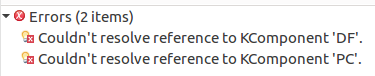
\includegraphics[width=3.90630in,height=0.79170in]{./Pictures/10000201000001770000004CA84119E1BC561581.png}\textbf{package}
components \{

\textbf{Component} PC \{

\textbf{port\_in} in \{\}

\textbf{port\_out} out \{\}

\}

\textbf{Component} DF \{

\textbf{port\_in} in \{\}

\textbf{port\_out} out \{\}

\textbf{port\_out} debug \{\}

\}

\}

\textbf{package} services \{

\textbf{service} MyService \{

\textbf{instance} pc : \emph{PC}

\textbf{instance} df : \emph{DF}

\}

\}

Xtext ermöglicht es, in seinem Standardverhalten jedes Element über
seinen vollen Namen analog zur Namensgebung von Java-Klassen
anzusprechen (alle Namen der Elemente im Baum mit „.`` voneinander
getrennt: z.B. „components.PC`` im Beispiel oben).

Eine \textbf{Referenz} in der \textbf{Grammatik }(z.B.
„{[}KComponent{]}``) wird jedoch standardmäßig über eine ID angesprochen
(ohne „.`` im Namen). Daher kann der volle Name nicht formuliert werden.
Möchte man dies ermöglichen, kann man wie folgt vorgehen:

...

KInstance: 'instance' name=ID ':'
type=\textbf{{[}}\emph{\textbf{KComponent}}\textbf{\textbar{}FQN{]}};

FQN \textbf{hidden}(): ID('.'ID)*; // allows
"\emph{packagename},\emph{componame}"

// (without spaces inbetween -- no WS hidden)

...

Damit kann man nun das obige Beispiel erfolgreich korrigieren:


\includegraphics[width=0.98350in,height=0.98350in]{./Pictures/1000020100000080000000807EA91CDFA7B7F397.png}...

\textbf{package} services \{

\textbf{service} MyService \{

\textbf{instance} pc : components.PC

\textbf{instance} df : components.DF

\}

\}

...

\subsection[Scoping
(Sichtbarkeit/Gültigkeit)]{\texorpdfstring{\protect\hypertarget{anchor-45}{}{}\protect\hypertarget{anchor-46}{}{}Scoping
(Sichtbarkeit/Gültigkeit)}{Scoping (Sichtbarkeit/Gültigkeit)}}\label{scoping-sichtbarkeitguxfcltigkeit}

Es gibt Fälle, bei denen es nicht erwünscht ist, eine beliebige Referenz
auf ein Objekt zu ermöglichen. Beispiele sind Methoden von
Objektinstanzen (z.B. bei Java) oder Ports von Instanzen (in unserem
Beispiel). Im ersten Beispiel möchte man nur Methoden einblenden, die
der Typ der Objektinstanz beinhaltet. Im zweiten Beispiel möchte man nur
Ports einblenden, die zur selektieren Instanz passen:

...

KService: 'service' name=ID '\{'

(

instances += KInstance\textbar{}

connections += KConnection

)*

'\}';

KConnection:

'connect'

srcInstance={[}\emph{KInstance}{]} '.' srcPort={[}\emph{KPortOut}{]}

'to'

dstInstance={[}\emph{KInstance}{]} '.' dstPort={[}\emph{KPortIn}{]}

;

...

Ohne weitere Anpassung wird folgender Code nicht akzeptiert (da die
Ports nicht sichtbar sind). Man könnte nun die Referenz auf die Ports
wie in Kapitel \protect\hyperlink{anchor-43}{8.1} realisieren, dies
würde jedoch keinen Zusammenhang zwischen den Ports und dem Typ der
Instanz berücksichtigen.

...

\textbf{service} MyService \{

\textbf{instance} pc : PC

\textbf{instance} df : DF

\textbf{connect} pc.\emph{out} \textbf{to} df.\emph{in} // Wunsch!

\}

...

Man kann nun diesen semantischen Zusammenhang „nur Ports zulassen, die
zum Typ der Instanz gehören`` wie folgt in das Modell einbringen: Man
definiert sich einen eigenen Scope-Provider (Geltungsbereich = Scope):
Öffnen Sie dazu die schon vorhandene Datei
kurs.xtext.dataflow.scoping.DataFlowDslScopeProvider und überladen Sie
die Methode „getScope`` (vgl. \protect\hyperlink{anchor-1}{/1/},
\protect\hyperlink{anchor-4}{/4/}):

\begin{itemize}
\tightlist
\item
  Hier kann man über eine „referenz`` das Attribut aus dem Modell in der
  Grammatik selektieren, für das ein neuer Gültigkeitsbereich definiert
  werden soll: In unserem Beispiel ist das die Referenz auf den
  Quell-Port („srcPort``) und Ziel-Port („dstPort``) der KConnection.
\item
  Weiter hat man den Zugriff über einen „context`` auf das betroffene
  Modellelement (hier die KConnection).
\item
  Hat man die Liste der gültigen Einträge erstellt, gibt man diese
  zurück (mithilfe der statischen Methode „Scopes.scopeFor``; siehe
  \protect\hyperlink{anchor-4}{/4/}).
\item
  Für alle Attribute, die man nicht gesondert behandeln möchte, gibt man
  das Ergebnis der Basisimplementierung zurück (vgl. Beispiel).
\end{itemize}

\textbf{class} DataFlowDslScopeProvider \textbf{extends}
AbstractDataFlowDslScopeProvider \{

\textbf{override} getScope(EObject context, EReference reference) \{

\textbf{if} (reference ==
DataFlowDslPackage.Literals.\emph{KCONNECTION\_\_SRC\_PORT}) \{

\textbf{val} kconn = context \textbf{as} KConnection;

\textbf{val} ports =
kconn.srcInstance.type.ports.\emph{filter}(KPortOut)

\textbf{return} Scopes.\emph{scopeFor}(ports);

\}

\textbf{else} \textbf{if} (reference ==
DataFlowDslPackage.Literals.\emph{KCONNECTION\_\_DST\_PORT}) \{

\textbf{val} kconn = context \textbf{as} KConnection;


\includegraphics[width=0.62800in,height=0.62800in]{./Pictures/1000020100000080000000807EA91CDFA7B7F397.png}\textbf{val}
ports = kconn.dstInstance.type.ports.\emph{filter}(KPortIn)

\textbf{return} Scopes.\emph{scopeFor}(ports);

\}

\textbf{super}.getScope(context, reference);

\}

\}

Aufgabe: Probieren Sie obiges Beispiel aus.

\subsection[Zusammenfassende erweiterte
Aufgabe]{\texorpdfstring{\protect\hypertarget{anchor-47}{}{}Zusammenfassende
erweiterte
Aufgabe}{Zusammenfassende erweiterte Aufgabe}}\label{zusammenfassende-erweiterte-aufgabe}

Testen Sie auch eine der folgenden (oder alle) Variationen des Beispiels
aus Abschnitt \protect\hyperlink{anchor-46}{8.2}:

\begin{itemize}
\item
  \textbf{Variation 1 „Ports mit Messages``}: Erlauben Sie „KMessages``
  in einem „KPackage`` zu definieren (Neues Modellelement mit Syntax
  „\textbf{Message \textless{}NAME\textgreater{}}``). Assoziieren Sie
  nun jeden Port mit einem KMessage und erlauben Sie nur Ports zu
  verknüpfen, die mit derselben Message assoziiert sind (siehe ein
  Beispiel eines solchen Modells unten).

  \begin{itemize}
  \tightlist
  \item
    \textbf{Lösung 1}: Modifizieren Sie den Scope Provider für den Ziel
    Port, um dort nur zum Quell Port passende Ports anzubieten (der
    Quell Port ist dann schon im Modell vorhanden -- andersherum gibt es
    Probleme)
  \item
    \textbf{Lösung 2}: Verwenden Sie die Modell Validierung (vgl.
    Abschnitt \protect\hyperlink{anchor-28}{5}) um lesbare
    Fehlermeldungen zu erzeugen.
  \end{itemize}
\item
  \textbf{Variation 2 „Vererbte Komponenten ``}: Erlauben Sie
  KComponenten \textbf{optional }von einer anderen KComponent
  „\textbf{abzuleiten}`` (Syntax: „Component A \textbf{extends B}
  \{...\}``. Nun sollen die „geerbten Ports`` ebenfalls angeboten
  werden.

  \begin{itemize}
  \tightlist
  \item
    Hinweis: Man kann Listen mit „+`` vereinen.
  \item
    Hinweis: Optionale Attribute in der Grammatik können mit „?``
    spezifiziert werden (vgl. \protect\hyperlink{anchor-3}{/3/}: such
    nach ‚\emph{as indicated by the ``?'' notation}`)
  \end{itemize}
\end{itemize}

Werden beide Variationen realisiert, ist folgende Eingabe möglich:


\includegraphics[width=0.98350in,height=0.98350in]{./Pictures/1000020100000080000000807EA91CDFA7B7F397.png}\textbf{package}
test1 \{

// Variation 1:

\textbf{Message} IQ\_Data

\textbf{Message} PC\_Data

\textbf{Message} PC\_DEBUG\_Data

\textbf{Message} DF\_Data

\textbf{Message} DF\_DEBUG\_Data

\textbf{Component} PC \{

\textbf{port\_in} pcin \{ IQ\_Data \} // Variation 1

\textbf{port\_out} pcout \{ PC\_Data \} // Variation 1

\textbf{port\_out} pcdbg \{ PC\_DEBUG\_Data \} // Variation 1

\}

\textbf{Component} ExPC \textbf{extends} PC \{ // Variation 2

\textbf{port\_out} pcout\_ex \{ PC\_Data \} // Variation 1

\}

\textbf{Component} DF \{

\textbf{port\_in} dfin \{ PC\_Data \} // Variation 1

\textbf{port\_in} dfdbg \{ PC\_DEBUG\_Data \} // ...

\textbf{port\_out} dfout \{ IQ\_Data \}

\textbf{port\_out} dfdbg \{ DF\_DEBUG\_Data \}

\}

\textbf{service} MyService \{

\textbf{instance} pc : ExPC

\textbf{instance} df : DF

\textbf{connect} pc.pcout\_ex \textbf{to} df.dfin // Variation 1

\textbf{connect} pc.pcdbg \textbf{to} df.dfdbg// Variation 1+2
(\emph{pcdbg} \emph{geerbt})

\}

\}

Code Generierung:

Versuchen Sie nun aus einem Modell wie dem Folgenden eine entsprechende
Ausgabe zu erzeugen (Das Modell kann mit oder ohne Messages vorliegen).
Kopieren Sie dazu die Ausgabe in Ihr Code Generator Skript (zwischen die
dreifachen Hochkommas) und ergänzen Sie sukzessive den Text mit Modell
Informationen, FOR-Schleifen, etc. (vgl. Abschnitt
\protect\hyperlink{anchor-33}{6}).

Diese Ausgabe kann man dann z.B. in \url{http://plantuml.com/} online
eingeben um sie in ein Bild umzuwandeln (oder man installiert das
PlantUML-Werkzeug):

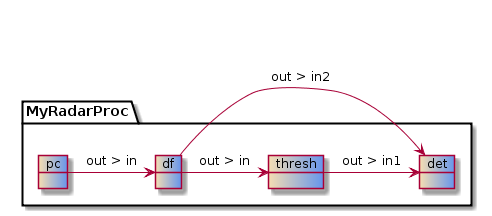
\includegraphics[width=5.19570in,height=1.71020in]{./Pictures/10000201000001EC000000D8D6389CC9995AC077.png}

\subsection[Modularisierung]{\texorpdfstring{\protect\hypertarget{anchor-48}{}{}Modularisierung}{Modularisierung}}\label{modularisierung}

In der Standardkonfiguration kann ein Modell jederzeit Modell Elemente
aus anderen Dateien anziehen, die im selben Projekt vorliegen.
Alternativ kann man auch fordern, dass ein speziell zu definierender
import Befehl verwendet wird, um andere Modell Dateien anzuziehen (dies
sind dann Modellelemente, die ein Attribut „\textbf{importURI}``
besitzten; dieses Attribut ist ein STRING, der eine andere Datei
lokalisiert). Das Vorgehen dafür ist in
\protect\hyperlink{anchor-4}{/4/} erklärt.

Das Einbinden anderer Modelle basierend auf anderen Metamodellen /
Grammatiken ist ebenfalls möglich. Dies erfordert jedoch weitere
Einstellungen. Für andere Grammatiken ist das Vorgehen in
\protect\hyperlink{anchor-4}{/4/} beschrieben.

\textbf{Optionale Aufgabe}: Teilen Sie Ihre Modelldatei auf. Probieren
Sie auch die Variante mit „importURI`` aus: Lesen Sie hier in
\protect\hyperlink{anchor-4}{/4/} nach, was zu tun ist (Stichwort:
„ImportUriGlobalScopeProvider``).

\section[Verschiedenes]{\texorpdfstring{\protect\hypertarget{anchor-49}{}{}Verschiedenes}{Verschiedenes}}\label{verschiedenes-1}

\subsection[Standalone Compiler für die eigene
DSL]{\texorpdfstring{\protect\hypertarget{anchor-50}{}{}Standalone
Compiler für die eigene
DSL}{Standalone Compiler für die eigene DSL}}\label{standalone-compiler-fuxfcr-die-eigene-dsl}

Um aus dem Java Projekt einen eigenständigen Compiler zu erzeugen, ist
wie folgt vorzugehen (Quelle: \protect\hyperlink{anchor-2}{/2/} und
persönliche Kommunikation mit \protect\hyperlink{anchor-1}{/1/}):

\begin{itemize}
\tightlist
\item
  In der mwe2-Datei (in unserem Beispiel
  src/kurs/xtext/dataflow/GenerateDataFlowDsl.mwe2) ist im Bereich
  „language`` folgender Code einzufügen: „fragment =
  generator.GeneratorFragment2 \{generateJavaMain = true\}``.
\end{itemize}

...

language = StandardLanguage \{

name = "org.example.xtext.fsm.FiniteStateMachine"

fileExtensions = "\emph{fsm}"

serializer = \{

generateStub = \textbf{false}

\}

validator = \{

// composedCheck =
"org.eclipse.xtext.validation.NamesAreUniqueValidator"

\}

fragment = generator.GeneratorFragment2 \{

generateJavaMain = \textbf{true}

\}

\}

\}

...

\begin{itemize}
\item
  Dann die Grammatik neu erzeugen.
\item
  Die neu erzeugte Klasse kurs.xtext.dataflow.generator.Main ausführen\\
  (Run As / Java Appplication). → Bricht mit einem Fehler (keine
  Eingabedateien) ab.

  \emph{Optional}: Man kann die Main Datei modifizieren, so dass sie
  nicht nur eine übergebene Datei „compiliert``, sondern auch viele
  Dateien (z.B. mit „*`` an der Konsole).
\item
  Abschließend mit „Rechts-Klick im Projekt Browser / Export`` das
  Projekt exportieren:

  \begin{itemize}
  \tightlist
  \item
    Selektion „\textbf{Runnable JAR File}``, „Next``
  \item
    \textbf{Launch Configuration}: „Main`` (das ist der Grund, dass man
    die Main 1x ausführen musste),\\
    \textbf{Export destination}: „mycompiler.jar``, 
  \item
    Selektion „\textbf{Package required libraries into generated JAR}``,
    „Finish``
  \end{itemize}
\end{itemize}

Mit dem so erzeugten Compiler („mycompiler.jar``) und den Modelldateien
kann man Modelle validieren und Code generieren:

pierre@solo2:\textasciitilde{}/demo\$ \textbf{ls}

mycompiler.jar test1.dataflow

pierre@solo2:\textasciitilde{}/demo\$ \textbf{java -jar mycompiler.jar
test1.dataflow }

Code generation finished.

pierre@solo2:\textasciitilde{}/demo\$ tree

\begin{itemize}
\item mycompiler.jar
\item src-gen
\begin{itemize}
\item Components1.txt
\item Components2.txt
\item Components3.txt
\item Components4.txt
\end{itemize}
\item test1.dataflow
\end{itemize}
1 directory, 6 files

Ist das Modell fehlerhaft oder erzeugt die Validierung eine Warnung
(vgl. Abschnitt \protect\hyperlink{anchor-30}{5.1}), wird kein Code
generiert (siehe Main.java):

pierre@solo2:\textasciitilde{}/demo\$ \textbf{java -jar mycompiler.jar
test1.dataflow }

WARNING:Name should start with a capital (test1.dataflow line : 10
column : 12)

pierre@solo2:\textasciitilde{}/demo\$

\subsection[Eclipse Plugins, Web Editoren mit
maven]{\texorpdfstring{\protect\hypertarget{anchor-51}{}{}Eclipse
Plugins, Web Editoren mit
maven}{Eclipse Plugins, Web Editoren mit maven}}\label{eclipse-plugins-web-editoren-mit-maven}

Die automatisch erstellte maven Projektstruktur beinhaltet folgende
Paktet

\begin{itemize}
\tightlist
\item
  „feature`` und „repository`` erstellen ein repository, welches als
  standalone wieder in eclipse installiert werden kann. 
\item
  „web`` erzeugt einen Webserver, der Anhand der DSL einen
  Webfrontendeditor bietet
\end{itemize}

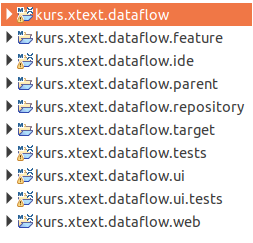
\includegraphics[width=2.63540in,height=2.53110in]{./Pictures/10000201000000FD000000F33F19609DDE80FED7.png}

Um die Projektstruktur via Kommandozeile zu bauen, kommt nun maven zum
Einsatz. Der Befehl „mvn clean verify`` im unten aufgeführten
Verzeichnis erzeugt den kompletten Projektbaum.

root@xtext:\textasciitilde{}/work/xtext-talks/kurs.xtext.dataflow.parent\$
mvn clean verify

...

{[}WARNING{]} No tests found.

{[}INFO{]}
-\/-\/-\/-\/-\/-\/-\/-\/-\/-\/-\/-\/-\/-\/-\/-\/-\/-\/-\/-\/-\/-\/-\/-\/-\/-\/-\/-\/-\/-\/-\/-\/-\/-\/-\/-\/-\/-\/-\/-\/-\/-\/-\/-\/-\/-\/-\/-\/-\/-\/-\/-\/-\/-\/-\/-\/-\/-\/-\/-\/-\/-\/-\/-\/-\/-\/-\/-\/-\/-\/-\/-

{[}INFO{]} Reactor Summary:

{[}INFO{]}

{[}INFO{]} kurs.xtext.dataflow.parent ......................... SUCCESS
{[} 0.081 s{]}

{[}INFO{]} kurs.xtext.dataflow ................................ SUCCESS
{[} 13.518 s{]}

{[}INFO{]} kurs.xtext.dataflow.ide ............................ SUCCESS
{[} 1.540 s{]}

{[}INFO{]} kurs.xtext.dataflow.ui ............................. SUCCESS
{[} 2.321 s{]}

{[}INFO{]} kurs.xtext.dataflow.web ............................ SUCCESS
{[} 3.302 s{]}

{[}INFO{]} kurs.xtext.dataflow.target ......................... SUCCESS
{[} 0.003 s{]}

{[}INFO{]} kurs.xtext.dataflow.feature ........................ SUCCESS
{[} 0.082 s{]}

{[}INFO{]} kurs.xtext.dataflow.repository ..................... SUCCESS
{[} 1.451 s{]}

{[}INFO{]} kurs.xtext.dataflow.tests .......................... SUCCESS
{[} 4.007 s{]}

{[}INFO{]} kurs.xtext.dataflow.ui.tests ....................... SUCCESS
{[} 7.859 s{]}

{[}INFO{]}
-\/-\/-\/-\/-\/-\/-\/-\/-\/-\/-\/-\/-\/-\/-\/-\/-\/-\/-\/-\/-\/-\/-\/-\/-\/-\/-\/-\/-\/-\/-\/-\/-\/-\/-\/-\/-\/-\/-\/-\/-\/-\/-\/-\/-\/-\/-\/-\/-\/-\/-\/-\/-\/-\/-\/-\/-\/-\/-\/-\/-\/-\/-\/-\/-\/-\/-\/-\/-\/-\/-\/-

{[}INFO{]} BUILD SUCCESS

{[}INFO{]}
-\/-\/-\/-\/-\/-\/-\/-\/-\/-\/-\/-\/-\/-\/-\/-\/-\/-\/-\/-\/-\/-\/-\/-\/-\/-\/-\/-\/-\/-\/-\/-\/-\/-\/-\/-\/-\/-\/-\/-\/-\/-\/-\/-\/-\/-\/-\/-\/-\/-\/-\/-\/-\/-\/-\/-\/-\/-\/-\/-\/-\/-\/-\/-\/-\/-\/-\/-\/-\/-\/-\/-

{[}INFO{]} Total time: 41.925 s

{[}INFO{]} Finished at: 2018-05-09T00:23:50+02:00

{[}INFO{]} Final Memory: 153M/1167M

{[}INFO{]}
-\/-\/-\/-\/-\/-\/-\/-\/-\/-\/-\/-\/-\/-\/-\/-\/-\/-\/-\/-\/-\/-\/-\/-\/-\/-\/-\/-\/-\/-\/-\/-\/-\/-\/-\/-\/-\/-\/-\/-\/-\/-\/-\/-\/-\/-\/-\/-\/-\/-\/-\/-\/-\/-\/-\/-\/-\/-\/-\/-\/-\/-\/-\/-\/-\/-\/-\/-\/-\/-\/-\/-

root@xtext:\textasciitilde{}/work/xtext-talks/kurs.xtext.dataflow.parent\$

\subsection[Import von maven
Projektstrukturen]{\texorpdfstring{\protect\hypertarget{anchor-52}{}{}Import
von maven
Projektstrukturen}{Import von maven Projektstrukturen}}\label{import-von-maven-projektstrukturen}

Mittels des maven Projektstruktur(pom.xml) und des m2e plugin von
eclipse ist es nun möglich, die Xtext Projekte ohne weiteren Aufwand zu
importieren.

\subsection[Templates]{\texorpdfstring{\protect\hypertarget{anchor-53}{}{}Templates}{Templates}}\label{templates}

Templates sind Textschnipsel, die man über Abkürzungen in ein Modell
einfügen kann.

Diese kann man am einfachsten in der Runtime-Workbench editieren (vgl.
\protect\hyperlink{anchor-13}{/11/}):

\begin{itemize}
\item
  Menu: ``Window/Preferences`` → „DataFlowDsl`` (Unsere Grammatik) →
  „Templates``
\item
  Hier kann man neue Templates anlegen: „New...``

  \begin{itemize}
  \tightlist
  \item
    Name: „NewComponent`` (Das ist das Kürzel, mit dem man den Code
    Schnipsel einfügen kann)
  \item
    Context: „KComponent``
  \item
    Description: „Add a new Component``
  \item
    Pattern (Hier kann man das meiste mit CTRL-Space vervollständigen):
  \end{itemize}
\end{itemize}

\begin{quote}
\textbf{Component} MyComponent \{
\end{quote}

\begin{quote}
\textbf{port\_in} myinput
\{\$\{message:CrossReference(KPort.message)\}\}
\end{quote}

\begin{quote}
\textbf{port\_out} myoutput \{
\$\{message:CrossReference(KPort.message)\}\}
\end{quote}

\begin{quote}
\}
\end{quote}

\begin{itemize}
\item
  \begin{itemize}
  \tightlist
  \item
    „OK``
  \end{itemize}
\end{itemize}

Probieren Sie das neue Template aus: Geben Sie in einem KPackage nun
„NewC``+CTRL-Space ein (damit selektieren Sie das neue Pattern
„NewComponent``).

Um die \textbf{Templates permanent zur Verfügung }zu \textbf{stellen},
muss man wie in \protect\hyperlink{anchor-13}{/11/} beschrieben
vorgehen:

\begin{itemize}
\tightlist
\item
  Im obigen Dialog die Templates exportieren (templates.xml).
\item
  Einen Ordner „templates`` im „UI``-Projekt anlegen.
\item
  Dort diesen neuen Ordner zu „bin.includes`` in den „build.properties``
  hinzufügen: \textbf{(1) }Doppel-Klick auf „build.properties`` Datei.
  \textbf{(2) }Haken beim Ordner „templates`` im Bereich „Binary Build``
  setzen.
\item
  Die exportierte Datei „templates.xml`` in diesen Ordner „templates``
  einfügen.
\item
  In der Datei „templates.xml`` zu den einzelnen Templates ein Attribut
  ‚id="ID\textless{}NUM\textgreater{}`` hinzufügen. 
\end{itemize}

Beispiel:

\textless{}?\emph{xml} version="1.0" encoding="UTF-8"
\emph{standalone}="no"?\textgreater{}\textless{}templates\textgreater{}\textless{}template
\textbf{id="ID1"} \emph{autoinsert}="true"
context="kurs.xtext.dataflow.DataFlowDsl.KComponent" deleted="false"
description="Add a new Component" enabled="true"
name="NewComponent"\textgreater{}Component MyComponent \{

port\_in \emph{myinput} \{\$\{message:CrossReference(KPort.message)\}\}

port\_out \emph{myoutput} \{
\$\{message:CrossReference(KPort.message)\}\}

\}\textless{}/template\textgreater{}\textless{}/templates\textgreater{}

\subsection[QualifiedNameProvider]{\texorpdfstring{\protect\hypertarget{anchor-54}{}{}QualifiedNameProvider}{QualifiedNameProvider}}\label{qualifiednameprovider}

Wir haben bereits gesehen, wie mittels Referenzen auf andere
Modellelemente anhand deren Namen (oder qualifizierenden Namen)
verwiesen wird. Existiert kein Name oder anderes Attribut, welches als
Referenz dient (oder soll der von Xtext erzeugt qualifizierende Name
angepasst werden), dann kann man mit minimalem Aufwand definieren, wie
dieser Name ermittelt wird.

Als Beispiel verwenden wir diesmal eine Sprache zur Definition von
Variablen und deren Initialisierung, deren Grammatik wie folgt definiert
ist:


\includegraphics[width=0.98350in,height=0.98350in]{./Pictures/1000020100000080000000807EA91CDFA7B7F397.png}\textbf{grammar}
kurs.xtext.VarLang \textbf{with} org.eclipse.xtext.common.Terminals

\textbf{generate} varLang "http://www.xtext.kurs/VarLang"

Model:

/* \emph{Ein} \emph{Modell} \emph{voller} \emph{Variablen} */

variable+=VariableInitialzation (';' variable+=VariableInitialzation)*;

VariableInitialzation:

/* \emph{Eine} \emph{Varable} \emph{besteht} \emph{wird}
\emph{deklariert} \emph{und} \emph{danach} \emph{einem} \emph{Wert}
\emph{zugewiesen}, \emph{der} in \emph{einem} \emph{Ausdruck}
\emph{definiert} \emph{wird} */

declaration = VariableDeclaration '=' value = Expression

;

VariableDeclaration:

/*EIne VariablenDeklaration \emph{besteht} \emph{aus} \emph{einem}
\emph{Typ} \emph{und} \emph{einem} \emph{Namen}*/

visibility=Type name = ID

;

\textbf{enum} Type:

/* \emph{Es} \emph{sind} \emph{nur} UINT32,UINT16 oder UINT 8 \emph{als}
\emph{Typen} \emph{erlaubt} */

UINT32='UINT32' \textbar{} UINT16='UINT16' \textbar{} UINT8='UINT8'

;

Expression:

/* \emph{Ein} \emph{Ausdruck} \emph{kann} \emph{aus} \emph{einem}
\emph{einzelnen} IntValue oder \emph{einer} \emph{Refrenz} \emph{auf}
\emph{eine} \emph{initialisierte} Variable \emph{bestehen}.

* \emph{Kann} \emph{ein} \emph{Ausdruck} die \emph{Summe} \emph{aus}
\emph{solchen} \emph{Elemente} \emph{beschreiben}. */

(value += IntValue \textbar{} value += VarReference) ( '+' (value +=
IntValue \textbar{} value += VarReference))*

;

IntValue:

/* IntValue \emph{enthält} \emph{einen} \emph{Ganzzahligen} \emph{Wert}
*/

value = INT

;

VarReference:

/* \emph{Eine} VariablenRefernz \emph{enthaält} \emph{eine}
\emph{Referenz} \emph{auf} \emph{eine} \emph{initialisierte} Variable
\emph{und} \emph{übernimmt} \emph{ihren}

* \emph{qualifizierenden} \emph{Namen} \emph{als} \emph{ihren}
\emph{eigenen} \emph{namen}.*/

name = {[}\emph{VariableInitialzation}{]}

;

Nach dem Erzeugen des Editors werden Eingaben wie

\textbf{UINT16} v1 = 1 + 1 ;

\textbf{UINT16} v2 = 1 + 2

bereits erfolgreich vom Parser erkannt. Versuchen wir jedoch stattdessen

\textbf{UINT16} v1 = 1 + 1 ;

\textbf{UINT16} v2 = 1 + v1

erhalten wir einen Fehler bei dem Verweis auf v1 in Zeile 2.

Die \textbf{Ursache für diesen Fehler }ist, dass die Referenz auf eine
\emph{VariableInitialzation} in der Grammatik-Regel VarReference von
Xtext nicht aufgelöst kann, weil VariableInitialzation weder einen
Namen, noch ein anderes Attribut hat, das als ein qualifizierender Name
dienen könnte.

\textbf{Lösung: }Wir können jedoch durch Überschreiben des von Xtext
verwendeten QualifiedNameProvider selbst bestimmen, wie der
qualifizierende Name eines Modellelements aussehen soll.

Dazu legen wir eine neue Xtend-Klasse
MyCustomQualifiedNameProvider.xtend an (Strg + N und dann nach „Xtend
Class`` filtern), diese kann z.B. im selben Package wie die *.xtext
Grammatik abgelegt werden (kurs.xtext).

Darin definieren wir, dass der qualifizierende Name einer
VariableInitialzation der Name der in

der enthaltenen VariableDeclaration sein soll:

\textbf{import}
org.eclipse.xtext.naming.DefaultDeclarativeQualifiedNameProvider

\textbf{import} kurs.xtext.varLang.VariableInitialzation;

\textbf{import} org.eclipse.xtext.naming.QualifiedName

\textbf{class} MyCustomQualifiedNameProvider \textbf{extends}
DefaultDeclarativeQualifiedNameProvider \{

\textbf{def} qualifiedName(VariableInitialzation initialization) \{

\textbf{return}
QualifiedName.\emph{create}(initialization.declaration.name);

\}

\}

anschließend müssen wir Xtext noch mitteilen, dass wir unseren eigenen
QualifiedNameProvider verwenden wollen, indem wir folgendes in der
VarLangRuntimeModule.xtend ergänzen:

...

\textbf{override} bindIQualifiedNameProvider() \{

/* \emph{weise} \emph{Xtext} an \emph{unseren} \emph{angepassten}
QualifiedNameSpaceProvider \emph{zu} \emph{nutzen} */

\textbf{return} MyCustomQualifiedNameProvider

\}

...

Nachdem wir den Editor neu generiert haben, wird nun das vorherige
Beispiel vom Parser erfolgreich erkannt:

\textbf{UINT16} v1 = 1 + 1 ;

\textbf{UINT16} v2 = 1 + v1

Wir können bei Bedarf auch das Standard Verhalten für die Erzeugung für
qualifizierende Namen von Xtext überschreiben (override statt def):

\textbf{override} qualifiedName(VariableInitialzation initialization) \{

\textbf{return}
QualifiedName.\emph{create}(initialization.declaration.name);

\}

\subsection[Zugriff auf Eltern Elemente im
AST]{\texorpdfstring{\protect\hypertarget{anchor-55}{}{}Zugriff auf
Eltern Elemente im
AST}{Zugriff auf Eltern Elemente im AST}}\label{zugriff-auf-eltern-elemente-im-ast}

Möchte man auf den besitzer eines Modell Elementes zugreifen, so ist
dies im AST (z.B. beom Code Generieren) über die Eigenschaft
„eConainer`` möglich. Das Ergebnis muss dann noch in den entsprechenden
Typ des der Eltern umgewalndet werden (e.eContainer as
ParentTypeAusGrammatik).

\section[Fazit]{\texorpdfstring{\protect\hypertarget{anchor-56}{}{}Fazit}{Fazit}}\label{fazit}

Dieses Dokument demonstriert, wie man mit relativ wenig Aufwand ein
Metamodell mittels Xtext spezifizieren kann, wie man Modelle validiert
und aus den Modellen Code generiert.

Die so erzeugten Modelle und Metamodelle gliedern sich nahtlos in die
EMF Welt ein. Dies erlaubt auf natürliche Weise eine Integration mit
anderen Werkzeugen und Formaten (z.B. ReqIF Format aus DOORS
(\url{https://eclipse.org/rmf/}, 2017/07), XMI UML Format aus Papyrus
(\url{https://eclipse.org/papyrus/}, 2017/07), \ldots{} und andere
hauseigene Modelle).

Besonders hervorzuheben ist die hohe Flexibilität textueller
Modellrepräsentationen:

\begin{itemize}
\tightlist
\item
  Einfach zu editieren (notfalls mit einem Texteditor).
\item
  Eingabe unvollständiger Modelle ist möglich.
\item
  Diff / Suchen-Ersetzen ist mit normalen Werkzeugen möglich.
\item
  Merge Aktivitäten sind einfach zu handeln (da die Modellrepräsentation
  auf Platte der gewohnten Eingabesyntax entspricht)
\item
  Volle Kompatibilität mit CI/CD (Build via commandline und Paketierung
  von Eclipse-Pluigns)
\end{itemize}

Wir hoffen es hat Spaß gemacht!

\end{document}
